\documentclass[11pt, openany]{article}

%%%%%%%%%%%%%%%%%%%%%%%%%%%%%% Loading packages that alter the style
\usepackage[]{graphicx}
\usepackage[]{color}
\usepackage{alltt}
\usepackage[T1]{fontenc}
\usepackage[utf8]{inputenc}
\setcounter{secnumdepth}{3}
\setcounter{tocdepth}{2}
\setlength{\parskip}{\smallskipamount}
\setlength{\parindent}{0pt}

% Set page margins
\usepackage[top=100pt,bottom=100pt,left=68pt,right=66pt]{geometry}

% Prevents LaTeX from filling out a page to the bottom
\raggedbottom

\usepackage[english]{babel}

% All page numbers positioned at the bottom of the page
\usepackage{fancyhdr}
\fancyhf{} % clear all header and footers
\fancyfoot[C]{\thepage}
\renewcommand{\headrulewidth}{0pt} % remove the header rule
\pagestyle{fancy}

% Changes the style of chapter headings
\usepackage{titlesec}
\titleformat{\chapter}
   {\normalfont\LARGE\bfseries}{\thechapter.}{1em}{}
% Change distance between chapter header and text
\titlespacing{\chapter}{0pt}{50pt}{2\baselineskip}

% Adds table captions above the table per default
\usepackage{float}
\floatstyle{plaintop}
\restylefloat{table}

% Adds space between caption and table
\usepackage[tableposition=top]{caption}

% Adds hyperlinks to references and ToC
\usepackage{hyperref}
\hypersetup{hidelinks,linkcolor = black} % Changes the link color to black and hides the hideous red border that usually is created

% If multiple images are to be added, a folder (path) with all the images can be added here 
\graphicspath{ {img/} }


%%%%%%%%%%%%%%%%%%%%%%%%%%%%%% Starts the document
\begin{document}

%%%%% Adds the title page
\begin{titlepage}
	\clearpage\thispagestyle{empty}
	\centering
	
	\vspace*{3cm}
	% Titles
	{\Huge \textbf{Schema Annotation Manual}} \\
	\vspace{1cm}
	{\normalsize Markus Neuwirth, % \\ specifies a new line
	             Ken D\'eguernel,
	             Christoph Finkensiep\par}
	\vspace{10cm}

    
\includegraphics[scale=0.6]{EPFL_logo.png}
    
    
	{\normalsize \'Ecole Polytechnique F\'ed\'erale de Lausanne \par}
		
	% Set the date
	{\normalsize \today \par}
	\vspace{2cm}
	
	\pagebreak
\end{titlepage}

% Adds a table of contents
\tableofcontents{}
\pagebreak


\section{General annotation guidelines}

\paragraph{How to read a schema prototype:\\}
The schema prototypes are represented by scale degrees, event by event and with voices ordered from bottom to top (from bass to soprano). For example, the prototype for the Do-Re-Mi schema with 4 voices is written as:
\begin{center}
\textbf{[[1, 3, 5, 1], [7, 4, 5, 2], [1, 3, 5, 3]]},
\end{center}
meaning that it is composed of three events, namely:
\begin{itemize}
\item 1\textsuperscript{st} event: \textbf{[1, 3, 5, 1]},
\item 2\textsuperscript{nd} event:\textbf{ [7, 4, 5, 2]},
\item 3\textsuperscript{rd} event: \textbf{[1, 3, 5, 3]}.
\end{itemize}
The first event consists of a 1\textsuperscript{st} scale degree in the bass, a 3\textsuperscript{rd} scale degree in the tenor, a 5\textsuperscript{th} scale degree in the alto, and again a 1\textsuperscript{st} scale degree in the soprano.\\

Each schema is given a unique designator that is structured as follows:
\begin{center}
\texttt{<schema name><number of voices><variant name>}
\end{center}
For example, the term \texttt{fonte.3.majmaj} is used to refer to the major/major variant of the three-voice realization of the Fonte schema (see below).

\paragraph{How to annotate:\\}
\begin{itemize}
\item For making the annotations see the instructions in the notebook. Note that you will need to add the annotations for each schema type separately. Therefore, we advise you to analyze a given piece first based on the printed score, where you add your annotations manually.
\item Please select the notes that belong to either the prototype of a particular schema or one of its variants as defined below.
If multiple pitches of the same pitch class are available as candidates, preferably select those pitches that are connected through the same register.
\item Annotate every instance of a given schema, even if it is a direct and/or literal repetition of an instance you have already annotated.
\item If you happen to come across schemata or schema variants not listed in the schema lexicon, please get in touch with one of the members of the project team.
\end{itemize}


\section{List of schemata}
Here is the list of schemata considered for the annotation, in alphabetical order:
\begin{itemize}
    \setlength\itemsep{1pt}
\item Ascending fifths sequence
\item Cadences
\item Ciacona
\item Descending fifths sequence
\item Do-Re-Mi
\item Fauxbourdon
\item Fenaroli
\item Folia
\item Fonte
\item Grand cadence
\item Half cadence
\item Indugio
\item Lamento
\item Le-Sol-Fi-Sol
\item Lully
\item Meyer
\item Monte
\item Morte
\item Omnibus
\item Pachelbel
\item Prinner
\item Quiescenza
\item Romanesca (galant)
\item Romanesca (old)
\item Sol-Fa-Mi
\item Teufelsmühle
\item Volta
\item Waldstein
\end{itemize}


\section{Schema description}


	\subsection{Ascending fifths sequence}
	
\subsubsection{Formal description:}
\begin{itemize}
\item Number of stages: 4-5
\item Number of voices: 2-4
\item Mode: major / minor
\item Harmonic signature: \texttt{I V ii vi iii}
\end{itemize}

\paragraph{Prototype:}
\begin{itemize}
\item 2 voices: \texttt{“ascfifths.2”} / \texttt{“ascfifths.2.min”}
	\begin{center}
    \textbf{[[1, 3], [5, 2], [2, 4], [6, 3], [3, 5]]}
    \end{center}
\item 3 voices: \texttt{“ascfifths.3”} / \texttt{“ascfifths.3.min”}
	\begin{center}
    \textbf{[[1, 1, 3], [5, 7, 2], [2, 2, 4], [6, 1, 3], [3, 3, 5]]}
    \end{center}
\item 4 voices: \texttt{“ascfifths.4”} / \texttt{“ascfifths.4.min”}
	\begin{center}
    \textbf{[[1, 5, 1, 3], [5, 5, 7, 2], [2, 6, 2, 4], [6, 6, 1, 3], [3, 7, 3, 5]]}
     \end{center}
\end{itemize}

\paragraph{Features:}
\begin{itemize}
\item Bass: leaping up a fifth and down a fourth
\item Soprano: alternating between step-wise motions and leaps in thirds
\item Often times with suspensions in the two upper voices added
\end{itemize}

\subsubsection{Examples:}
\begin{center}
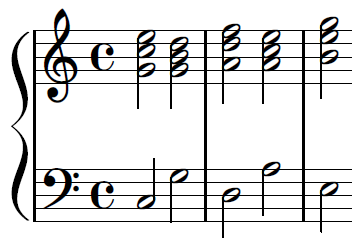
\includegraphics[scale=0.5]{asc5th.png}
\end{center}



	\subsection{Cadences}


	\subsection{Ciacona}

\subsubsection{Formal description:}
\begin{itemize}
\item Number of stages: 4
\item Number of voices: 2-4
\item Mode: major / minor
\item Harmonic signature: \texttt{I V6 viio6/V V}
\end{itemize}

\paragraph{Prototype:}
\begin{itemize}
\item 2 voices: \texttt{“ciacona.2”} / \texttt{“ciacona.2.min”}
	\begin{center}	
	\textbf{[[1, 5], [7, 5], [6, $\sharp$4], [5, 5]]}
	\end{center}
\item 3 voices: \texttt{“ciacona.3”} / \texttt{“ciacona.3.min”}
	\begin{center}	
	\textbf{[[1, 3, 5], [7, 2, 5], [6, 1, $\sharp$4], [5, 7, 5]]}
	\end{center}
\end{itemize}

\paragraph{Features:}
\begin{itemize}
\item Bass: fills the tetrachord 1-5 in diatonically descending steps
\item Middle voice: shadows the bass in parallel thirds or tenths
\item Soprano: carries out a soprano clausula
\item Effect of light tonicization of the dominant (see also Tenorizans Half Cadence)
\item Similarity with the diatonic Lamento
\end{itemize}

\subsubsection{Examples:}


	\subsection{Descending fifths sequence}
	
\subsubsection{Formal description:}
\begin{itemize}
\item Number of stages: 3 or more
\item Number of voices: 2-4
\item Mode: major / minor
\item Harmonic signature: \texttt{V/x x}
\end{itemize}

\paragraph{Prototype:}
\begin{itemize}
\item 2 voices: \texttt{“descfifths.2”} / \texttt{“descfifths.2.min”}
	\begin{center}
    \textbf{[[1, 3], [4, 4], [7, 2], [3, 3]]}
    \end{center}
\item 3 voices: \texttt{“descfifths.3”} / \texttt{“descfifths.3.min”}
	\begin{center}
    \textbf{[[1, 5, 3], [4, 6, 4], [7, 4, 2], [3, 5, 3]]}
    \end{center}
\item 4 voices: \texttt{“descfifths.4”} \texttt{“descfifths.4.min”}
\end{itemize}

\paragraph{Features:}
\begin{itemize}
\item Melody: stepwise
\item Bass: leaping or stepwise
\end{itemize}

\subsubsection{Examples:}


	\subsection{Do-Re-Mi}
	
\subsubsection{Formal description:}
\begin{itemize}
\item Number of stages: 3
\item Number of voices: 2-4
\item Mode: major / minor
\item Harmonic signature: \texttt{I V (V) I}
\end{itemize}

\paragraph{Prototype:}
\begin{itemize}
\item 2 voices: \texttt{“doremi.2”} / \texttt{“doremi.2.min”}
	\begin{center}
    \textbf{[[1, 1], [7, 2], [1, 3]]}
    \end{center}
\item 3 voices: \texttt{“doremi.3”} / \texttt{“doremi.3.min”}
	\begin{center}
    \textbf{[[1, 3, 1], [7, 5, 2], [1, 5, 3]]}
    \end{center}
\item 4 voices: \texttt{“doremi.4”} / \texttt{“doremi.4.min”}
	\begin{center}
    \textbf{[[1, 3, 5, 1], [7, 4, 5, 2], [1, 3, 5, 3]]}
    \end{center}
\end{itemize}

\paragraph{Features:}
\begin{itemize}
\item Three events (potentially) equally spaced (or with an extended first stage)
\item 1-2-3 stepwise ascent in the melody with possible chromatic passing tones
\item Sometimes realized in a pairwise fashion: Do-Re // Re-Mi
\item 1-7-1 (sometimes 7 substituted by 5) in the bass
\end{itemize}

\paragraph{Variants:}
\begin{itemize}
\item With cadential 5-1 bass:  \texttt{“doremi.2.cadbass”} / \texttt{“doremi.2.cadbassmin”}
	\begin{center}
    \textbf{[[1, 1], [5, 2], [1, 3]]}
    \end{center}
\end{itemize}

\subsubsection{Examples:}
\begin{itemize}
\item Leclair, Opus 1, no.3, mvt. 2, Allegro (1723)
\begin{center}
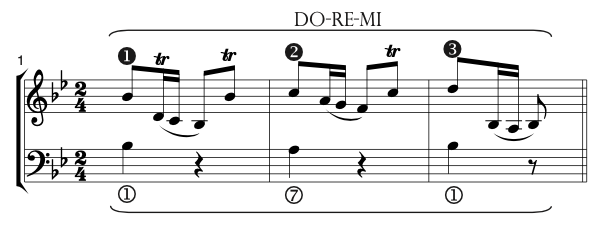
\includegraphics[scale=0.5]{leclair1.png}
\end{center}
\item Cimarosa, Sonata C56, Allegro, (1780s)
\begin{center}
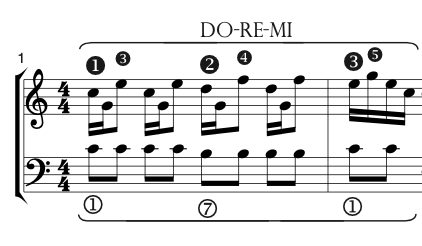
\includegraphics[scale=0.5]{cimarosa56.png}
\end{center}
\item Mozart, Horn Concerto (K. 447), mvt. 3, Allegro (1791)
\begin{center}
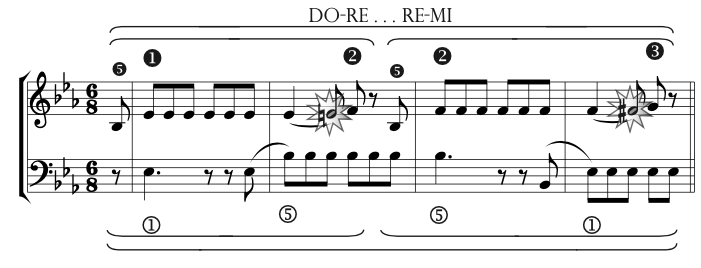
\includegraphics[scale=0.5]{mozart447.png}
\end{center}
\end{itemize}


	\subsection{Fauxbourdon}
	
\subsubsection{Formal description:}
\begin{itemize}
\item Number of stages: 3-7; not fixed in the prototype
\item Number of voices: 3
\item Mode: major / minor
\item Harmonic signature: e.g., \texttt{viio6 I6 ii6 iii6 IV6 V6 vi6} (ascending or descending)
\end{itemize}

\paragraph{Prototype ascending:}
\begin{itemize}
\item 3 voices: \texttt{“fauxbourdon.3.asc”} / \texttt{“fauxbourdon.3.asc.min”}
	\begin{center}
	\textbf{[[2, 4, 7], [3, 5, 1], [4, 6, 2], [5, 7, 3], [6, 1, 4], [7, 2, 5], [1, 3, 6]]}
    \end{center}
\end{itemize}

\paragraph{Prototype descending:}
\begin{itemize}
\item 3 voices: \texttt{“fauxbourdon.3.desc”} / \texttt{“fauxbourdon.3.desc.min”}
	\begin{center}
	\textbf{[[1, 3, 6], [7, 2, 5], [6, 1, 4], [5, 7, 3], [4, 6, 2], [3, 5, 1], [[2, 4, 7]]}
    \end{center}
\end{itemize}

\paragraph{Features:}
\begin{itemize}
\item The fauxbourdon consists either of the whole sequence of chords or of a subset of adjacent chords that may vary in length.
\item Can be played either upwards or downwards (or a mixture of both)
\item Potentially elaborated by suspensions
\item Potentially chromatized
\end{itemize}

\subsubsection{Examples:}
\begin{itemize}
\item Beethoven, Piano Sonata in C op. 2 No. 3, final mvt., opening (1796)
\begin{center}
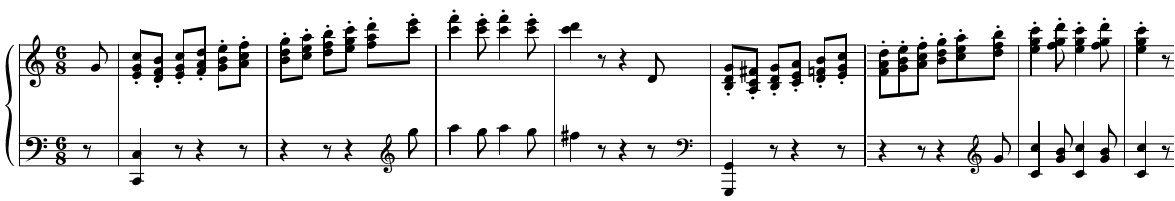
\includegraphics[scale=0.6]{beethoven2.png}
\end{center}
\end{itemize}


	\subsection{Fenaroli}
	
\subsubsection{Formal description:}
\begin{itemize}
\item Number of stages: 4
\item Number of voices: 2-4
\item Mode: major / minor
\item Harmonic signature: \texttt{V65 I V43 I6}
\end{itemize}

\paragraph{Prototype:}
\begin{itemize}
\item 2 voices: \texttt{“fenaroli.2”} / \texttt{“fenaroli.2.min”}
	\begin{center}
	\textbf{[[7, 4], [1, 3], [2, 7], [3, 1]]}
	\end{center}
\item 3 voices: \texttt{“fenaroli.3”} / \texttt{“fenaroli.3.min”}
	\begin{center}
	\textbf{[[7, 5, 4], [1, 5, 3], [2, 5, 7], [3, 5, 1]]}
	\end{center}
\item 4 voices: \texttt{“fenaroli.4”} / \texttt{“fenaroli.4.min”}
	\begin{center}
	\textbf{[[7, 5, 6, 4], [1, 3, 5, 3], [2, 3, 6, 7], [3, 3, 6, 1]]}
	\end{center}
\end{itemize}

\paragraph{Features:}
\begin{itemize}
\item The four events, equally spaced, are usually played twice.
\item Bass: follows a 7-1-2-3 movement.
\item Melody: usually follows a 4-3-7-1. Sometimes played as 2-3-7-1 to create a canon with the bass.
\end{itemize}

\paragraph{Variants:}
\begin{itemize}
\item Bass/Melody inversion: \texttt{“fenaroli.2.flipped”} / \texttt{“fenaroli.2.flippedmin”}
	\begin{center}
	\textbf{[[4, 7], [3, 1], [7, 2], [1, 3]]}
	\end{center}
\item Canon-like melody, 2 voices: \texttt{“fenaroli.2.melcanon”} / \texttt{“fenaroli.2.melcanonmin”}
	\begin{center}
	\textbf{[[7, 2], [1, 3], [2, 7], [3, 1]]}
	\end{center}
\item Canon-like melody, 3 voices: \texttt{“fenaroli.3.melcanon”} / \texttt{“fenaroli.3.melcanonmin”}
	\begin{center}
	\textbf{[[7, 5, 2], [1, 5, 3], [2, 5, 7], [3, 5, 1]]}
	\end{center}
\item Canon-like bass: \texttt{“fenaroli.2.basscanon”} / \texttt{“fenaroli.2.basscanonmin”}
	\begin{center}
	\textbf{[[7, 4], [1, 3], [4, 7], [3, 1]]}
	\end{center}
\item Full Durante: \texttt{“fenaroli.2.durante”} / \texttt{“fenaroli.2.durantemin”}
	\begin{center}
	\textbf{[[7, 5], [7, 4], [1, 3], [1, 1], [2, 7], [2, 5], [3, 1], [3, 3]]}
	\end{center}
\end{itemize}

\subsubsection{Examples:}
\begin{itemize}
\item Durante, Studio no.1, mvt. 1, (1747)
\begin{center}
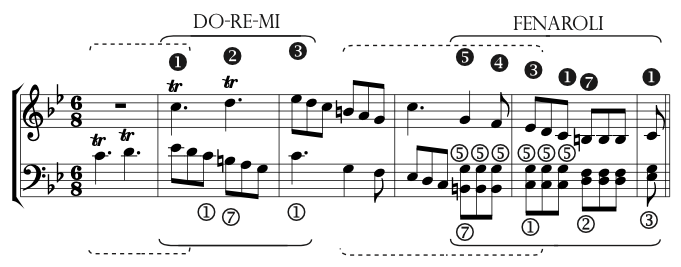
\includegraphics[scale=0.5]{durante1.png}
\end{center}
\item Cimarosa, Sonata C51, Allegro (1780s)
\begin{center}
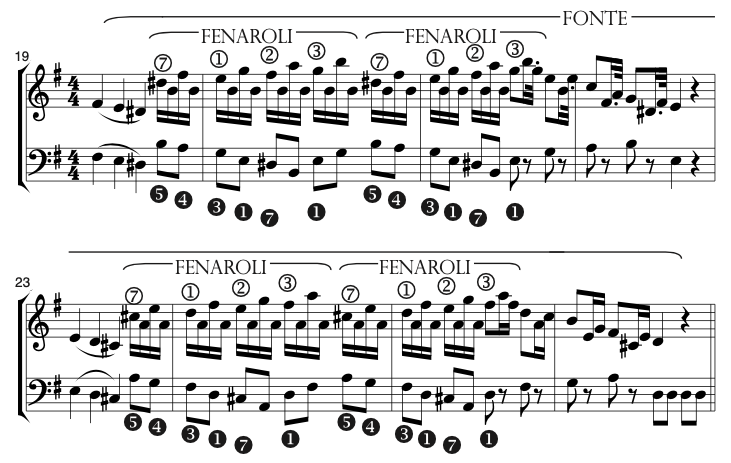
\includegraphics[scale=0.5]{cimarosa51.png}
\end{center}
\end{itemize}


	\subsection{Folia}
	
\subsubsection{Formal description:}
\begin{itemize}
\item Number of stages: 4; fixed in the prototype
\item Number of voices: 2-4
\item Mode: minor
\item Harmonic signature: \texttt{V i V/III III}
\end{itemize}

\paragraph{Prototype:}
\begin{itemize}
\item 2 voices: \texttt{“folia.2”}
	\begin{center}
	\textbf{[[5, 7], [1, 1], [$\flat$7, 2], [3, 3]]}
	\end{center}
\item 3 voices: \texttt{“folia.3”}
	\begin{center}
	\textbf{[[5, 7, 2], [1, 1, 3], [$\flat$7, 2, 4], [3, 3, 5]]}
	\end{center}
\item 4 voices: \texttt{“folia.4”}
	\begin{center}
	\textbf{[[5, 5, 7, 2], [1, 5, 1, 3], [$\flat$7, $\flat$7, 2, 4], [3, $\flat$7, 3, 5]]}
	\end{center}
\end{itemize}

\paragraph{Features:}
\begin{itemize}
\item Soprano: moves linearly and ascending
\item Bass: alternates between upward leaps (by fourth) and descending steps (by second)
\item The schema is followed by the “old” Romanesca (typically the combination of both is referred to as “Folia”)
\end{itemize}

\subsubsection{Examples:}
\begin{center}
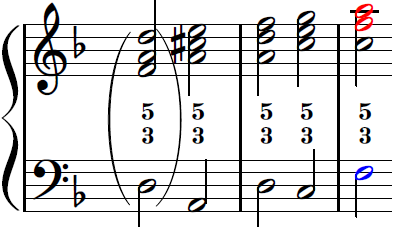
\includegraphics[scale=0.8]{folia.png}
\end{center}


	\subsection{Fonte}
	
\subsubsection{Formal description:}
\begin{itemize}
\item Number of stages: 4; fixed in the prototype
\item Number of voices: 2-4
\item Mode: major / minor
\item Harmonic signature: \texttt{V65/ii ii V65 I}
\end{itemize}

\paragraph{Prototype:}
\begin{itemize}
\item 2 voices: \texttt{“fonte.2”}
	\begin{center}
	\textbf{[[$\sharp$1, 5], [2, 4], [7, 4], [1, 3]]}
	\end{center}
\item 3 voices: \texttt{“fonte.3”}
	\begin{center}
	\textbf{[[$\sharp$1, 6, 5], [2, 6, 4], [7, 5, 4], [1, 5, 3]]}
	\end{center}
\item 4 voices: \texttt{“fonte.4”}
	\begin{center}
	\textbf{[[$\sharp$1, 6, 3, 5], [2, 6, 2, 4], [7, 5, 2, 4], [1, 5, 1, 3]]}
	\end{center}
\end{itemize}

\paragraph{Features:}
\begin{itemize}
\item Four events presented as two pairs
\item First half in minor, and second half in major one whole-tone lower
\item Melody: short scale-wise descent
\item Bass: usually ascends from leadings tones (7-1); sometimes 5-1 or 2-1
\end{itemize}

\paragraph{Variants:}
\begin{itemize}
\item Inversion soprano/bass, 2 voices: \texttt{“fonte.2.flipped”}
	\begin{center}
	\textbf{[[5, $\sharp$1], [4, 2], [4, 7], [3, 1]]}
	\end{center}
\item Inversion soprano/bass, 3 voices: \texttt{“fonte.3.flipped”}
	\begin{center}
	\textbf{[[5, 6, $\sharp$1], [4, 6, 2], [4, 5, 7], [3, 5, 1]]}
	\end{center}
\item with cadential basses: \texttt{“fonte.2.cadbass”}
	\begin{center}
	\textbf{[[6, 5], [2, 4], [5, 4], [1, 3]]}
	\end{center}
\item with (2-1) basses, tenorizans, 2 voices: \texttt{“fonte.2.tenbass”}
	\begin{center}
	\textbf{[[3, 5], [2, 4], [2, 4], [1, 3]]}
	\end{center}
\item with (2-1) basses, tenorizans, 3 voices: \texttt{“fonte.3.tenbass”}
	\begin{center}
	\textbf{[[3, $\sharp$1, 5], [2, 2, 4], [2, 7, 4], [1, 1, 3]]}
	\end{center}
\item Voice-exchange, 2 voices: \texttt{“fonte.2.voiceex”}
	\begin{center}
	\textbf{[[$\sharp$1, 5], [2, 4], [5, $\sharp$1], [4, 2], [7, 4], [1, 3], [4, 7], [3, 1]]}
	\end{center}
\item Voice-exchange, 3 voices: \texttt{“fonte.3.voiceex”}
	\begin{center}
	\textbf{[[$\sharp$1, 6, 5], [2, 6, 4], [5, 6, $\sharp$1], [4, 6, 2], [7, 5, 4], [1, 5, 3], [4, 5, 7], [3, 5, 1]]}
	\end{center}
\item Major-major, 2 voices: \texttt{“fonte.2.majmaj”}
	\begin{center}
	\textbf{[[$\sharp$1, 5], [2, $\sharp$4], [7, 4], [1, 3]]}
	\end{center}
\item Major-major, 3 voices: \texttt{“fonte.3.majmaj”}
	\begin{center}
	\textbf{[[$\sharp$1, 6, 5], [2, 6, $\sharp$4], [7, 5, 4], [1, 5, 3]]}
	\end{center}
\item Chromatic variant, 2 voices: \texttt{“fonte.2.chromatic”}
	\begin{center}
	\textbf{[[$\sharp$1, $\flat$7], [2, 6], [7, $\flat$6], [1, 5]]}
	\end{center}
\item Chromatic variant, 3 voices: \texttt{“fonte.3.chromatic”}
	\begin{center}
	\textbf{[[$\sharp$1, 5, $\flat$7], [2, 4, 6], [7, 4, $\flat$6], [1, 3, 5]]}
	\end{center}
\item Minor-minor, 2 voices: \texttt{“fonte.2.minmin”}
	\begin{center}
	\textbf{[[$\sharp$1, 5], [2, 4], [7, 4], [1, $\flat$3]]}
	\end{center}
\item Minor-minor, 3 voices: \texttt{“fonte.3.minmin”}
	\begin{center}
	\textbf{[[$\sharp$1, 6, 5], [2, 6, 4], [7, 5, 4], [1, 5, $\flat$3]]}
	\end{center}
\item Phrygian, 2 voices: \texttt{“fonte.2.phrygian”}
	\begin{center}
	\textbf{[[$\flat$7, 5], [6, 5], [$\flat$6, 4], [5, 4], [1, 3]]}
	\end{center}
\item Phrygian, 3 voices: \texttt{“fonte.3.phrygian”}
	\begin{center}
	\textbf{[[$\flat$7, 2, 5], [6, $\sharp$1, 5], [$\flat$6, 1, 4], [5, 7, 4], [1, 1, 3]]}
	\end{center}
\item Seventh chords, 2 voices: \texttt{“fonte.2.seventh”}
	\begin{center}
	\textbf{[[6, 5], [2, $\sharp$4], [5, 4], [1, 3]]}
	\end{center}
\item Seventh chords, 3 voices: \texttt{“fonte.3.seventh”}
	\begin{center}
	\textbf{[[6, $\sharp$1, 5], [2, 1, $\sharp$4], [5, 7, 4], [1, 1, 3]]}
	\end{center}
\end{itemize}

\begin{center}
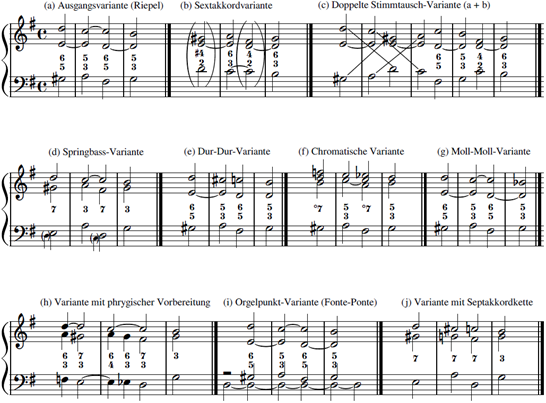
\includegraphics[scale=1]{fontevar.png}
\end{center}

\subsubsection{Examples:}
\begin{itemize}
\item Pasquali, Opus 1, no.2, mvt. 3 (1744)
\begin{center}
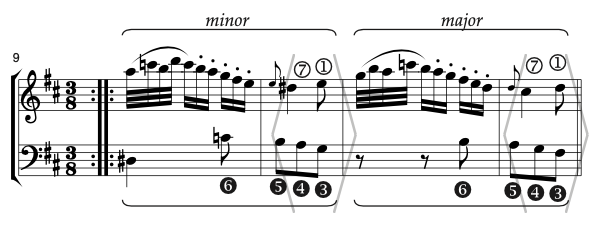
\includegraphics[scale=0.5]{pasquali1.png}
\end{center}
\item Gluck, Trio Sonatas, no.5, mvt.1 (1746)
\begin{center}
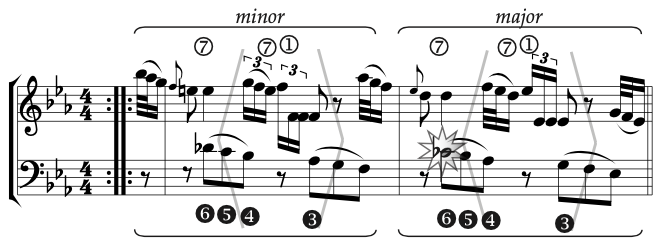
\includegraphics[scale=0.5]{gluck5.png}
\end{center}
\item Wodiczka, Opus 1, no.2, mvt.3 (1739)
\begin{center}
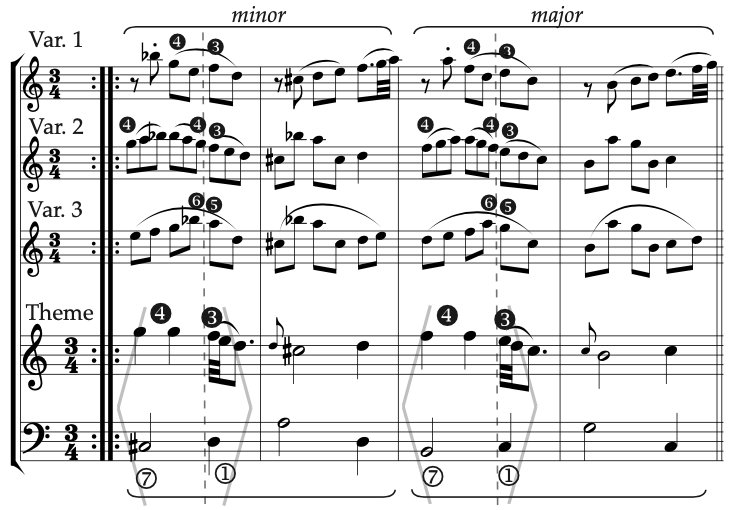
\includegraphics[scale=0.5]{wodiczka1.png}
\end{center}
\end{itemize}


	\subsection{Grand cadence}
	
\subsubsection{Formal description:}
\begin{itemize}
\item Number of stages: 4-5
\item Number of voices: 2-4
\item Mode: major / minor
\item Harmonic signature: \texttt{I6 ii6 V(64) V7 I}
\end{itemize}

\paragraph{Prototype:}
\begin{itemize}
\item 2 voices: \texttt{“grandcad.2”} / \texttt{“grandcad.2.min”}
	\begin{center}
	\textbf{[[3, 1], [4, 6], [5, 5], [1, 1]]}
	\end{center}
\item 2 voices: \texttt{“grandcad.2.long”} / \texttt{“grandcad.2.longmin”}
	\begin{center}
	\textbf{[[3, 1], [4, 6], [5, 5], [5, 2], [1, 1]]}
	\end{center}
\end{itemize}

\paragraph{Features:}
\begin{itemize}
\item Melody: Descent from a higher 1 to a lower 1 following 1-6-5-2-1
\item Bass: 3-4-5 ascent followed with a cadential 5-1
\end{itemize}

\subsubsection{Examples:}
\begin{itemize}
\item Clementi, Opus 4, no.5, mvt.2, Allegretto (1780)
\begin{center}
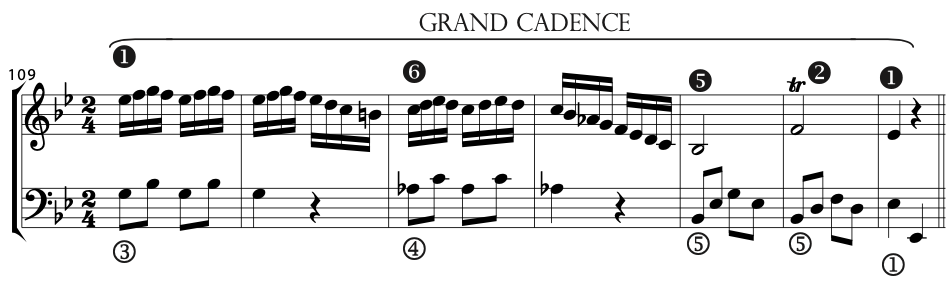
\includegraphics[scale=0.5]{clementi4.png}
\end{center}
\item Dittersdorf, String Quintet K.190, no.6, mvt.1 (1789)
\begin{center}
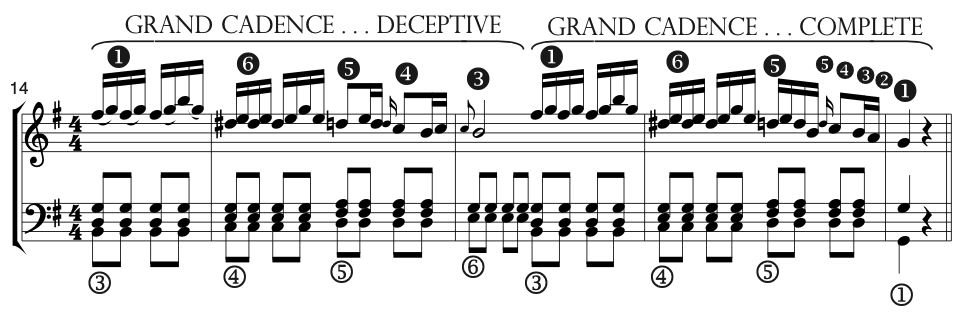
\includegraphics[scale=0.5]{dittersdorf190.png}
\end{center}
\end{itemize}

	
	\subsection{Half cadence}

\subsubsection{Formal description:}
\begin{itemize}
\item Number of stages: 3
\item Number of voices: 3-4
\item Mode: major / minor
\item Harmonic signature: \texttt{I6 ii6 V}
\end{itemize}


\paragraph{Variants:}
\begin{itemize}
\item Converging half cadence: \texttt{“halfcadconv.3”}
	\begin{center}
	\textbf{[[4, 6, 2], [$\sharp$4, 6, 1], [5, 5, 7]]}
	\end{center}
\item Phrygian half cadence: \texttt{“halfcadphryg.3”}
	\begin{center}
	\textbf{[[6, 1, 4], [$\flat$6, 1, $\sharp$4], [5, 7, 5]]}
	\end{center}
\item Tenorizans half cadence: \texttt{“halfcadten.3”}
	\begin{center}
	\textbf{[[1, 3, 5], [6, 1, $\sharp$4], [5, 7, 5]]}
	\end{center}
\item Simple half cadence: \texttt{“halfcadsim.4”}
	\begin{center}
	\textbf{[[7, 5, 2, 4], [1, 5, 1, 3], [5, 5, 7, 2]]}
	\end{center}
\end{itemize}


	\subsection{Indugio}
	
\subsubsection{Formal description:}
\begin{itemize}
\item Number of stages: 4
\item Number of voices: 2-3
\item Mode: major / minor
\item Harmonic signature: \texttt{ii65 I64 IV6 I64}
\end{itemize}

\paragraph{Prototype:}
\begin{itemize}
\item 2 voices: \texttt{“indugio.2”} / \texttt{“indugio.2.min”}
	\begin{center}
	\textbf{[[4, 2], [5, 3], [6, 4], [5, 3]]}
	\end{center}
\item 3 voices: \texttt{“indugio.3”} / \texttt{“indugio.3.min”}
	\begin{center}
	\textbf{[[4, 1, 2], [5, 1, 3], [6, 1, 4], [5, 1, 3]]}
	\end{center}
\end{itemize}

\paragraph{Features:}
\begin{itemize}
\item Sustained tonic note as an innervoice pedal
\item Sixth interval between outer-voices moving in a linear fashion
\item Often repeated (looplike)
\item Pattern can start on any of the predominant instances (\texttt{ii65, IV, IV6})
\end{itemize}

\paragraph{Variants:}
\begin{itemize}
\item IV chord variant, 2 voices: \texttt{“indugio.2.voiceex”} / \texttt{“indugio.2.voiceexmin”}
	\begin{center}
	\textbf{[[4, 6], [3, 5], [6, 4], [5, 3]]}
	\end{center}
\item IV chord variant, 3 voices: \texttt{“indugio.3.voiceex”} / \texttt{“indugio.3.voiceexmin”}
	\begin{center}
	\textbf{[[4, 1, 6], [3, 1, 5], [6, 1, 4], [5, 1, 3]]}
	\end{center}
\item Preparamento alla cadenza, 3 voices: \texttt{“indugio.3.prepallacad“}
	\begin{center}
	\textbf{[[4, 1, 6], [5, 1, 5], [6, 1, 4], [5, 1, 5]]}
	\end{center}
\end{itemize}

\subsubsection{Examples:}
\begin{center}
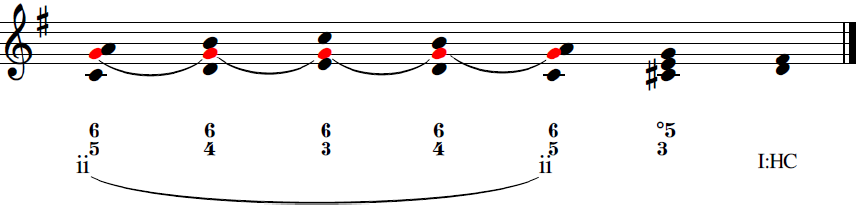
\includegraphics[scale=0.5]{indugio1.png}\\
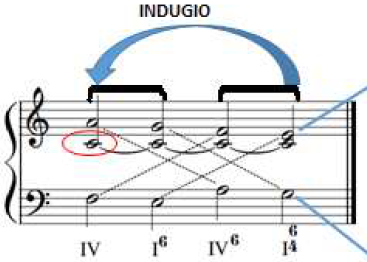
\includegraphics[scale=0.5]{indugio2.png}\\
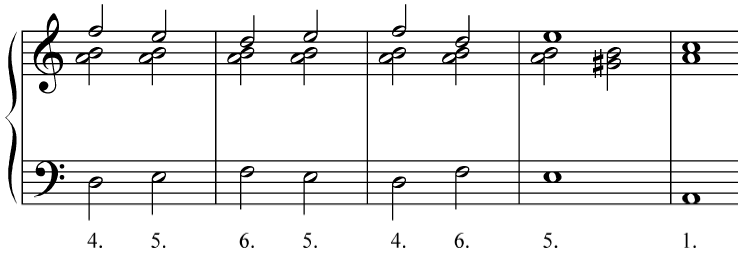
\includegraphics[scale=0.5]{indugio3.png}
\end{center}
\begin{itemize}
\item Cimarosa, Sonata C70, Andantino (1780s)
\begin{center}
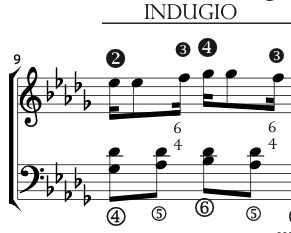
\includegraphics[scale=0.5]{cimarosa70.png}
\end{center}
\item Cimarosa, Sonata C72, Allegro (1780s)
\begin{center}
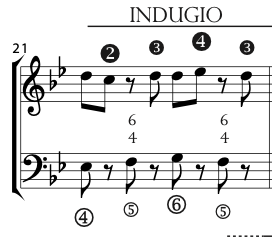
\includegraphics[scale=0.5]{cimarosa72.png}
\end{center}
\end{itemize}


	\subsection{Lamento}
	
\subsubsection{Formal description:}
\begin{itemize}
\item Number of stages: 4
\item Number of voices: 2-4
\item Mode: minor
\item Harmonic signature: \texttt{i v6 iv6 V}
\end{itemize}

\paragraph{Prototype:}
\begin{itemize}
\item 2 voices: \texttt{“lamento.2”}
	\begin{center}
	\textbf{[[1, 3], [7, 2], [6, 1], [5, 7]]}
	\end{center}
\item 3 voices: \texttt{“lamento.3”}
	\begin{center}
	\textbf{[[1, 3, 5], [7, 2, 5], [6, 1, 4], [5, 7, 5]]}
	\end{center}
\end{itemize}

\paragraph{Features:}
\begin{itemize}
\item Two voices moving in parallel thirds or tenths
\item Typically ends on a half cadence (Phrygian type)
\end{itemize}

\subsubsection{Examples:}


	\subsection{Le-Sol-Fi-Sol}
	
\subsubsection{Formal description:}
\begin{itemize}
\item Number of stages: 4
\item Number of voices: 2-4
\item Mode: minor
\item Harmonic signature: \texttt{VI i64 $\sharp$viio7/V V}
\end{itemize}

\paragraph{Prototype:}
\begin{itemize}
\item 2 voices: \texttt{"lesolfisol.2"}
	\begin{center}
	\textbf{[[6, 3], [5, 3], [$\sharp$4, 3], [5, 2]]}
	\end{center}
\item 3 voices: \texttt{"lesolfisol.3"}
	\begin{center}
	\textbf{[[6, 1, 3], [5, 1, 3], [$\sharp$4, 1, 3], [5, 7, 2]]}
	\end{center}
\end{itemize}

\paragraph{Features:}
\begin{itemize}
\item The upper voices sustain their notes until they resolve at the end
\item Bass moves chromatically around scale degree 5
\end{itemize}

\subsubsection{Examples:}


	\subsection{Lully}
	
\subsubsection{Formal description:}
\begin{itemize}
\item Number of stages: 4; fixed in the prototype
\item Number of voices: 2-4
\item Mode: major / minor
\item Harmonic signature: \texttt{I ii42 V65 I}
\end{itemize}

\paragraph{Prototype:}
\begin{itemize}
\item 2 voices: \texttt{"lully.2"} / \texttt{"lully.2.min"}
	\begin{center}
	\textbf{[[1, 3], [1, 2], [7, 2], [1, 3]]}
	\end{center}
\item 3 voices: \texttt{"lully.3"} / \texttt{"lully.3.min"}
	\begin{center}
	\textbf{[[1, 1, 3], [1, 2, 4], [7, 2, 4], [1, 1, 3]]}
	\end{center}
\item 4 voices: \texttt{"lully.4"} / \texttt{"lully.4.min"}
	\begin{center}
	\textbf{[[1, 5, 1, 3], [1, 6, 2, 4], [7, 5, 2, 4], [1, 5, 1, 3]]}
	\end{center}
\end{itemize}

\paragraph{Features:}
\begin{itemize}
\item Melody: the melody typically arrives at scale degree 3, either by linear ascent or descent, or by a neighboring motion.
\item Bass: The bass moves from 1 to 7 because it is turned into a dissonance by the upper voices; it then returns to 1.
\item The tonal effect is tonic prolongation.

\end{itemize}

\subsubsection{Examples:}
\begin{center}
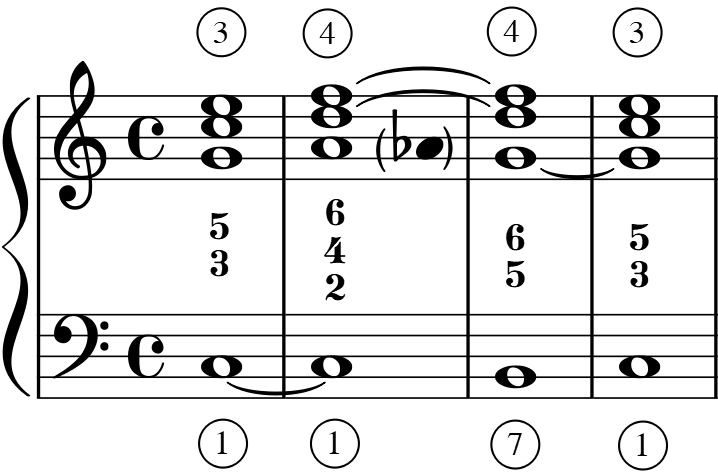
\includegraphics[scale=0.3]{lully.png}
\end{center}


	\subsection{Meyer}
	
\subsubsection{Formal description:}
\begin{itemize}
\item Number of stages: 4; fixed in the prototype
\item Number of voices: 2-4
\item Mode: major / minor
\item Harmonic signature: \texttt{I V43 V65 I}
\end{itemize}

\paragraph{Prototype:}
\begin{itemize}
\item 2 voices: \texttt{“meyer.2”} / \texttt{“meyer.2.min”}
	\begin{center}
	\textbf{[[1, 1], [2, 7], [7, 4], [1, 3]]}
	\end{center}
\item 4 voices: \texttt{“meyer.4”} / \texttt{“meyer.4.min”}
	\begin{center}
	\textbf{[[1, 3, 5, 1], [2, 3, 6, 7], [7, 5, 6, 4], [1, 3, 5, 3]]}
	\end{center}
\end{itemize}

\paragraph{Features:}
\begin{itemize}
\item Four events presented as two pairs at analogous positions in the metrical grid.
\item Melody: descending semitones 1-7 answered by 4-3
\item Bass: ascending step 1-2 answered by 7-1 (or 5-1)
\end{itemize}

\paragraph{Variants:}
\begin{itemize}
\item 5-1 bass: \texttt{“meyer.2.cadbass”} / \texttt{“meyer.2.cadbassmin”}
	\begin{center}
	\textbf{[[1, 1], [2, 7], [5, 4], [1, 3]]}
	\end{center}
\item Jupiter: \texttt{“meyer.2.jupiter”} / \texttt{“meyer.2.jupitermin”}
	\begin{center}
	\textbf{[[1, 1], [2, 2], [7, 4], [1, 3]]}
	\end{center}
\item Pastorella: \texttt{“meyer.2.pastorella”} / \texttt{“meyer.2.pastorellamin”}
	\begin{center}
	\textbf{[[1, 3], [2, 2], [7, 4], [1, 3]]}
	\end{center}
\item Aprile: \texttt{“meyer.2.aprile”}
	\begin{center}
	\textbf{[[1, 1], [2, 7], [7, 2], [1, 1]]}
	\end{center}
\end{itemize}

\subsubsection{Examples:}
\begin{itemize}
\item Haydn, Symphony in Bb (Hob. I:35), mvt.1, Allegro di molto (1767)
\begin{center}
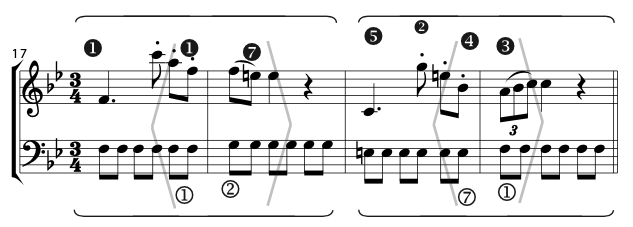
\includegraphics[scale=0.5]{haydn35.png}
\end{center}
\item Dittersdorf, Symphony in C (K.1), mvt.1, Allegro moderato (1766)
\begin{center}
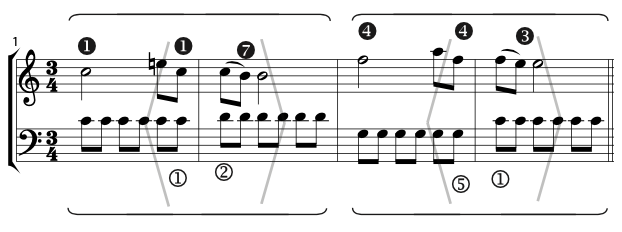
\includegraphics[scale=0.5]{dittersdorf1.png}
\end{center}
\item Mozart, Symphony KV551 “Jupiter”, mvt. 4, Molto allegro (1788)
\begin{center}
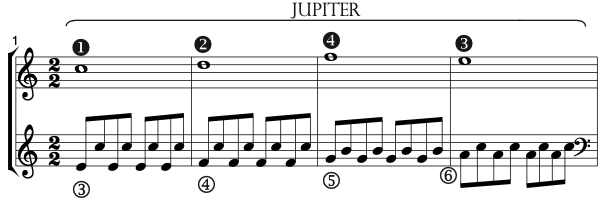
\includegraphics[scale=0.5]{mozart551.png}
\end{center}
\item Gossec, Missa pro defunctis, mvt. 15, Andante (1760)
\begin{center}
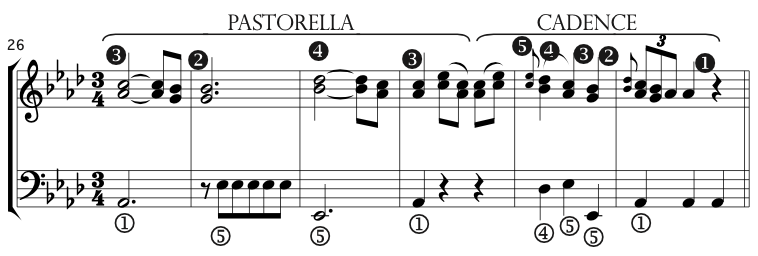
\includegraphics[scale=0.5]{gossecmpd.png}
\end{center}
\end{itemize}


	\subsection{Monte}
	
\subsubsection{Formal description:}
\begin{itemize}
\item Number of stages: 4; fixed in the prototype
\item Number of voices: 2-4
\item Mode: major / minor
\item Harmonic signature: \texttt{I6 IV ii6 V}
\end{itemize}

\paragraph{Prototype:}
\begin{itemize}
\item 2 voices (short): \texttt{“monte.2”}
	\begin{center}
	\textbf{[[3, $\flat$7], [4, 6], [$\sharp$4, 1], [5, 7]]}
	\end{center}
\item 3 voices (short): \texttt{“monte.3”}
	\begin{center}
	\textbf{[[3, 5, $\flat$7], [4, 4, 6], [$\sharp$4, 6, 1], [5, 5, 7]]}
	\end{center}
\item 2 voices (long): \texttt{“monte.2.long”}
	\begin{center}
	\textbf{[[3, 1], [3, $\flat$7], [4, 6], [$\sharp$4, 2], [$\sharp$4, 1], [5, 7]]}
	\end{center}
\item 3 voices (long): \texttt{“monte.3.long”}
	\begin{center}
	\textbf{[[3, 5, 1], [3, 5, $\flat$7], [4, 4, 6], [$\sharp$4, 6, 2], [$\sharp$4, 6, 1], [5, 5, 7]]}
	\end{center}
\end{itemize}

\paragraph{Features:}
\begin{itemize}
\item Two main sections, the second one a step higher the the first. The first one is presenting the subdominant, the second one the dominant.
\item Bass: consecutive chromatic ascents from leading tones to local tonics.
\item Melody: local descents complementing the bass
\item Relation to the 5-6 progression
\end{itemize}

\subsubsection{Examples:}
\begin{center}
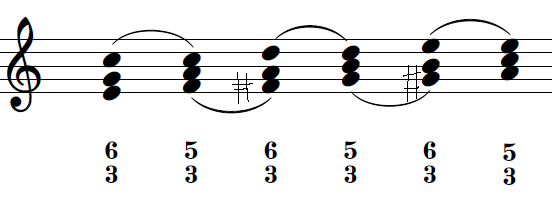
\includegraphics[scale=0.5]{monte.png}
\end{center}
\begin{itemize}
\item Clementi, Op.4, no.5, mvt.2, Allegretto (1780)
\begin{center}
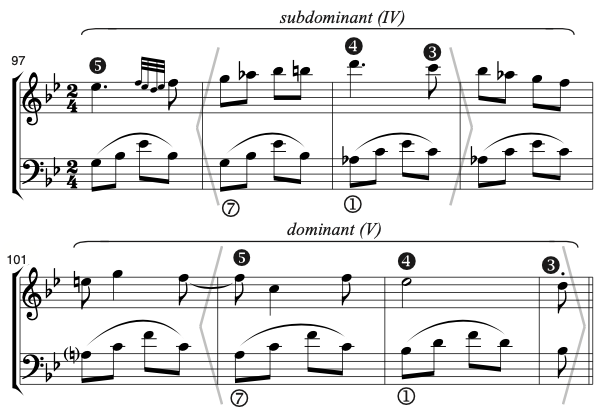
\includegraphics[scale=0.5]{clementi4b.png}
\end{center}
\item Durante, Studio no.6, Adagio (1747)
\begin{center}
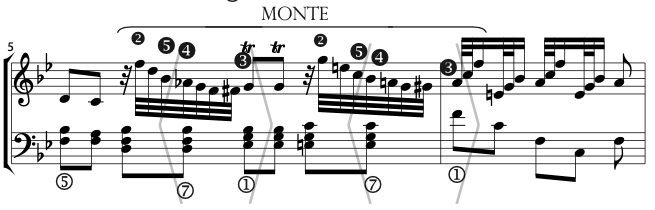
\includegraphics[scale=0.5]{durante6.png}
\end{center}
\item Wodiczka, Op.1, no.1, mvt.1, Largo (1739)
\begin{center}
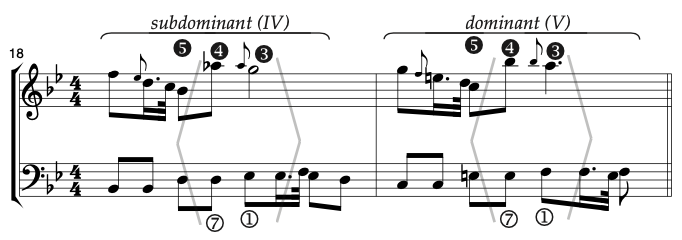
\includegraphics[scale=0.5]{wodiczka1b.png}
\end{center}
\end{itemize}


	\subsection{Morte}
	
\subsubsection{Formal description:}
\begin{itemize}
\item Number of stages: 5
\item Number of voices: 2-4
\item Mode: minor
\item Harmonic signature: \texttt{i V2/iv IV6 Ger6 V(64)}
\end{itemize}

\paragraph{Prototype:}
\begin{itemize}
\item 2 voices: \texttt{“morte.2”}
	\begin{center}
	\textbf{[[1, 3], [$\flat$7, $\sharp$3], [$\sharp$6, 4], [6, $\sharp$4], [5, 5]]}
	\end{center}
\item 3 voices: \texttt{“morte.3”}
	\begin{center}
	\textbf{[[1, 1, 3], [$\flat$7, 1, $\sharp$3], [$\sharp$6, 1, 4], [6, 1, $\sharp$4], [5, 1, 5]]}
	\end{center}
\end{itemize}

\paragraph{Features:}
\begin{itemize}
\item Soprano: chromatically ascending
\item Bass: chromatically descending.
\item Close relation to the Omnibus
\end{itemize}

\subsubsection{Examples:}
\begin{center}
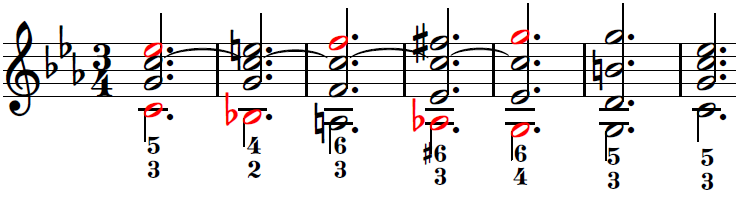
\includegraphics[scale=0.8]{morte.png}
\end{center}


	\subsection{Omnibus}
	
\subsubsection{Formal description:}
\begin{itemize}
\item Number of stages: 6; fixed in the prototype
\item Number of voices: 2-3
\item Mode: minor
\item Harmonic signature: \texttt{V7 vii64 V42 V7/vi $\sharp$v64 V42/vi}
\end{itemize}

\paragraph{Prototype:}
\begin{itemize}
\item 2 voices: \texttt{“omnibus.2”}
	\begin{center}
	\textbf{[[5, 4], [$\sharp$4, $\sharp$4], [4, 5], [3, $\sharp$5], [$\sharp$2, $\sharp$5], [2, $\sharp$5]]}
	\end{center}
\item 3 voices: \texttt{“omnibus.3”}
	\begin{center}
	\textbf{[[5, 2, 4], [$\sharp$4, 2, $\sharp$4], [4, 2, 5], [3, 2, $\sharp$5], [$\sharp$2, $\sharp$2, $\sharp$5], [2, 3, $\sharp$5]]}
	\end{center}
\end{itemize}

\paragraph{Features:}
\begin{itemize}
\item Bass: chromatically descending
\item Soprano: chromatically ascending
\item Inner voice(s): sustained
\end{itemize}

\subsubsection{Examples:}
\begin{center}
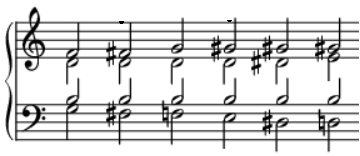
\includegraphics[scale=1]{omnibus.png}
\end{center}


	\subsection{Pachelbel}
	
\subsubsection{Formal description:}
\begin{itemize}
\item Number of stages: 4-6
\item Number of voices: 2
\item Mode: major / minor
\item Harmonic signature: \texttt{I V vi iii (IV I)}
\end{itemize}

\paragraph{Prototype:}
\begin{itemize}
\item 2 voices: \texttt{“pachelbel.2”}
	\begin{center}
	\textbf{[[1, 3], [5, 2], [6, 1], [3, 7]]}
	\end{center}
\item 3 voices: \texttt{“pachelbel.3”}
	\begin{center}
	\textbf{[[1, 5, 3], [5, 7, 2], [6, 3, 1], [3, 5, 7]]}
	\end{center}
\item 2 voices (long): \texttt{“pachelbel.2.long”}
	\begin{center}
	\textbf{[[1, 3], [5, 2], [6, 1], [3, 7], [4, 6], [1, 5]]}
	\end{center}
\item 3 voices (long): \texttt{“pachelbel.3.long”}
	\begin{center}
	\textbf{[[1, 5, 3], [5, 7, 2], [6, 3, 1], [3, 5, 7], [4, 1, 6], [1, 3, 5]]}
	\end{center}
\end{itemize}

\paragraph{Features:}
\begin{itemize}
\item Four (or six) events, typically equally spaced
\item Bass: Usually follows a 1-5-6-3(-4-1) movement. Sometimes realized stepwise (1-7-6-5(-4-3))
\item Melody: Stepwise descent 3-2-1-7(-6-5)
\end{itemize}

\paragraph{Variants:}
\begin{itemize}
\item Stepwise bass, 2 voices: \texttt{“pachelbel.2.stepwise”}
	\begin{center}
	\textbf{[[1, 3], [7, 2], [6, 1], [5, 7]]}
	\end{center}
\item Stepwise bass, 3 voices: \texttt{“pachelbel.3.stepwise”}
	\begin{center}
	\textbf{[[1, 5, 3], [7, 5, 2], [6, 3, 1], [5, 3, 7]]}
	\end{center}
\item Stepwise bass (long), 2 voices: \texttt{“pachelbel.2.stepwiselong”}
	\begin{center}
	\textbf{[[1, 3], [7, 2], [6, 1], [5, 7], [4, 6], [3, 5]]}
	\end{center}
\item Stepwise bass (long), 3 voices: \texttt{“pachelbel.3.stepwiselong”}
	\begin{center}
	\textbf{[[1, 5, 3], [7, 5, 2], [6, 3, 1], [5, 3, 7], [4, 1, 6], [3, 1, 5]]}
	\end{center}
\item Chromatic, 3 voices: \texttt{“pachelbel.3.chromatic”}
	\begin{center}
	\textbf{[[1, 1, 3], [$\sharp$5, 7, 2], [6, 6, 1], [3, 5, $\flat$7], [4, 4, 6]]}
	\end{center}
\item Chromatic (long), 3 voices: \texttt{“pachelbel.3.chromaticlong”}
	\begin{center}
	\textbf{[[1, 1, 3], [3, 1, 3], [$\sharp$4, 1, 2], [$\sharp$5, 7, 2], [6, 7, 1], [1, 6, 1], [2, 6, $\flat$7], [3, 5, $\flat$7], [4, 5, 6]]}
	\end{center}
\end{itemize}

\subsubsection{Examples:}
\begin{itemize}
\item Pachelbel, Canon in D Major, (1680s)
\begin{center}
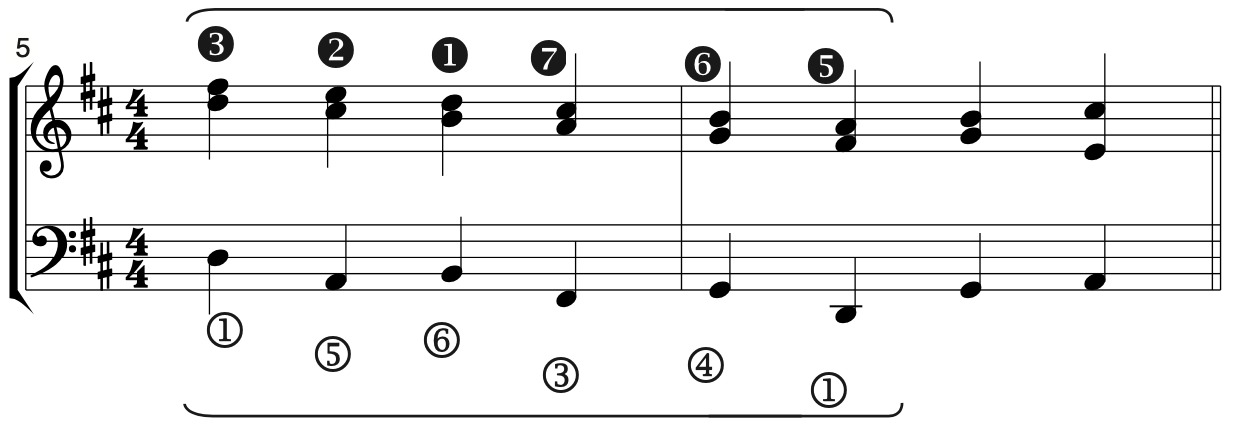
\includegraphics[scale=0.5]{pachelbelcanon.png}
\end{center}
\item Handel, Exercises for Princess Anne, Allegro (1724)
\begin{center}
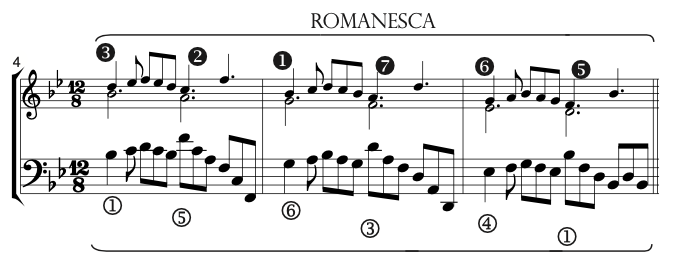
\includegraphics[scale=0.5]{handelanne.png}
\end{center}
\item Schobert, Opus 6, no.1, mvt.1, Andante (1761)
\begin{center}
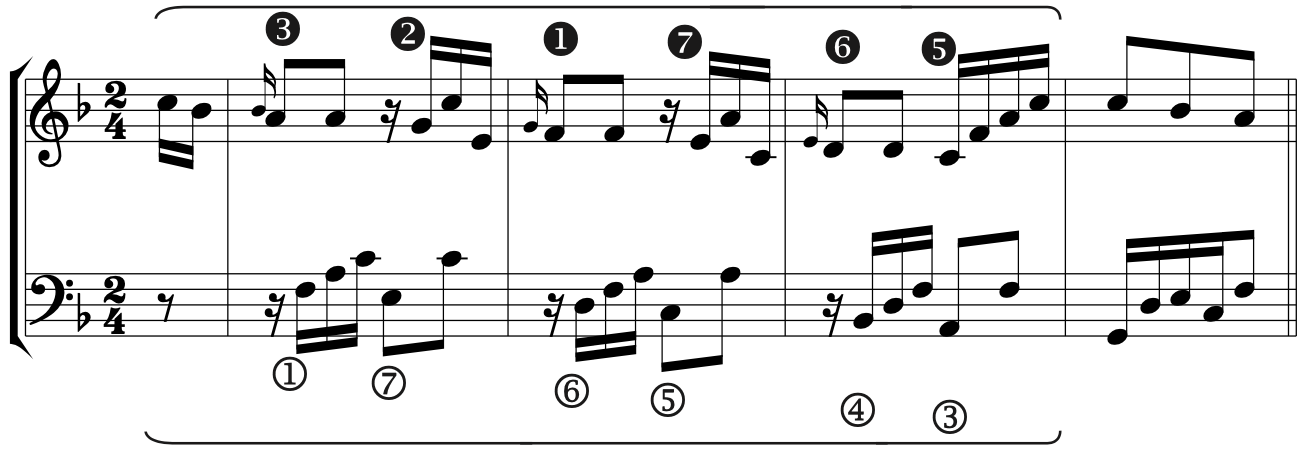
\includegraphics[scale=0.5]{schobert6.png}
\end{center}
\end{itemize}


	\subsection{Prinner}
	
\subsubsection{Formal description:}
\begin{itemize}
\item Number of stages: 4; fixed in the prototype
\item Number of voices: 2-3
\item Mode: major
\item Harmonic signature: \texttt{IV I6 viio6 I}
\end{itemize}

\paragraph{Prototype:}
\begin{itemize}
\item 2 voices: \texttt{"prinner.2"}
	\begin{center}
	\textbf{[[4, 6], [3, 5], [2, 4], [1, 3]]}
	\end{center}
\item 3 voices: \texttt{"prinner.3"}
	\begin{center}
	\textbf{[[4, 1,  6], [3, 1, 5], [2, 7, 4], [1, 1, 3]]}
	\end{center}
\end{itemize}

\paragraph{Features:}
\begin{itemize}
\item Four events with equal spacing or with an extended third stage.
\item Melody: stepwise descent 6-5-4-3 (sometimes 6-5-4-2-3 for a stronger cadence)
\item Bass: stepwise descent 4-3-2-1 (sometimes 4-3-2-1 for a stronger cadence)
\end{itemize}

\paragraph{Variants:}
\begin{itemize}
\item First inversion 2 voices: \texttt{“prinner.2.flipped”}
	\begin{center}
	\textbf{[[4, 1], [3, 1], [2, 7], [1, 1]]}
	\end{center}
\item First inversion 3 voices: \texttt{“prinner.3.flipped”}
	\begin{center}
	\textbf{[[4, 6, 1], [3, 5, 1], [2, 4, 7], [1, 3, 1]]}
	\end{center}
\item Second inversion 2 voices: \texttt{“prinner.2.tenorflipped”}
	\begin{center}
	\textbf{[[1, 6], [1, 5], [7, 4], [1, 3]]}
	\end{center}
\item Second inversion 3 voices: \texttt{“prinner.3.tenorflipped”}
	\begin{center}
	\textbf{[[1, 4, 6], [1, 3, 5], [7, 2, 4], [1, 1, 3]]}
	\end{center}
\end{itemize}

\subsubsection{Examples:}
\begin{itemize}
\item Wodiczka, Opus 1, no. 3, mvt. 1, Adagio (1739)
\begin{center}
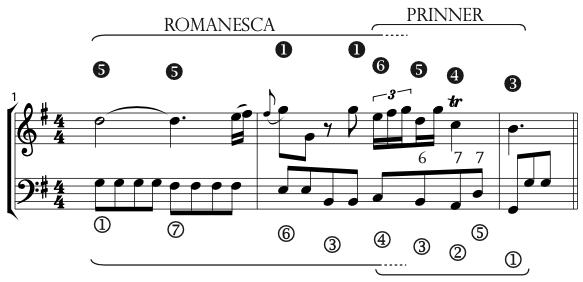
\includegraphics[scale=0.5]{wodiczka1c.png}
\end{center}
\item Zingarelli, Partimento in C Major (1790s)
\begin{center}
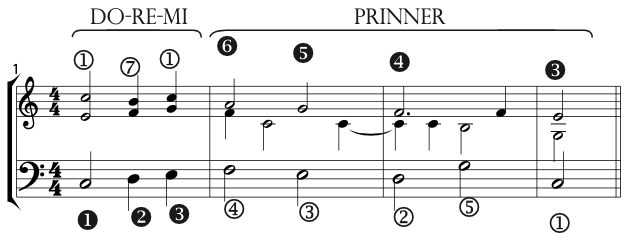
\includegraphics[scale=0.5]{zingarelliparti.png}
\end{center}
\end{itemize}


	\subsection{Quiescenza}
	
\subsubsection{Formal description:}
\begin{itemize}
\item Number of stages: 4; fixed in the prototype
\item Number of voices: 2-4
\item Mode: major
\item Harmonic signature: \texttt{I(V7/IV IV viio6 I)}
\end{itemize}

\paragraph{Prototype:}
\begin{itemize}
\item 2 voices: \texttt{“quiescenza.2”}
	\begin{center}
	\textbf{[[1, $\flat$7], [1, 6], [1, 7], [1, 1]]}
	\end{center}
\item 3 voices: \texttt{“quiescenza.3”}
	\begin{center}
	\textbf{[[1, 3, $\flat$7], [1, 4, 6], [1, 2, 7], [1, 3, 1]]}
	\end{center}
\end{itemize}

\paragraph{Features:}
\begin{itemize}
\item The four events are usually played twice in succession.
\item In the soprano voice, the descending whole tone ($\flat$7-6) is answered by the ascending semitone (natural 7-1)
\item Pedal on 1 in the bass (or a figuration reiterating 1)
\end{itemize}

\paragraph{Variants:}
\begin{itemize}
\item Diatonic type: \texttt{“quiescenza.2.diatonic”}
	\begin{center}
	\textbf{[[1, 5], [1, 6], [1, 7], [1, 1]]}
	\end{center}
\item Diatonic type: \texttt{“quiescenza.2.diatonic”}
	\begin{center}
	\textbf{[[1, 3, 5], [1, 4, 6], [1, 2, 7], [1, 3, 1]]}
	\end{center}
\end{itemize}

\subsubsection{Examples:}
\begin{itemize}
\item Gaviniés, Op.3, no.5, mvt.3, Tempo di Minuetto (1764)
\begin{center}
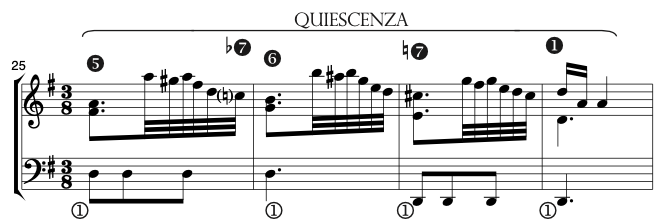
\includegraphics[scale=0.5]{gavinies3.png}
\end{center}
\item Wanhal, Quartet in F Major (F6), mvt.1, Allegro moderato (1771)
\begin{center}
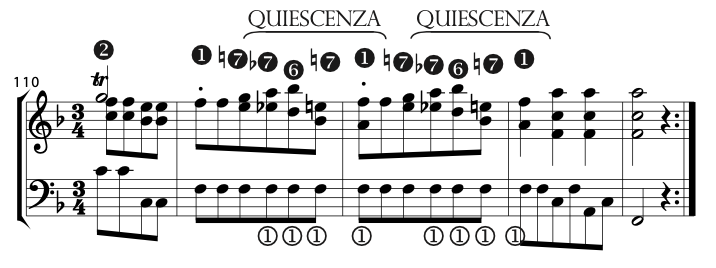
\includegraphics[scale=0.5]{wanhal6.png}
\end{center}
\item D. Scarlatti, Sonata K.250 (1740)
\begin{center}
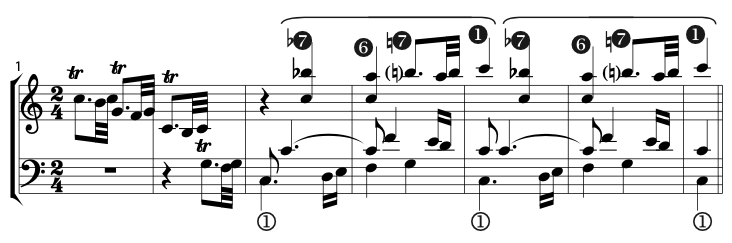
\includegraphics[scale=0.5]{scarlatti250.png}
\end{center}
\end{itemize}


	\subsection{Romanesca (Galant)}
	
\subsubsection{Formal description:}
\begin{itemize}
\item Number of stages: 4; fixed in the prototype
\item Number of voices: 2
\item Mode: major
\item Harmonic signature: \texttt{I V6 vi I6}
\end{itemize}

\paragraph{Prototype:}
\begin{itemize}
\item 2 voices: \texttt{“romanescagalant.2”}
	\begin{center}
	\textbf{[[1, 1], [7, 5], [6, 1], [3, 1]]}
	\end{center}
\item 3 voices: \texttt{“romanescagalant.3”}
	\begin{center}
	\textbf{[[1, 5, 1], [7, 2, 5], [6, 3, 1], [3, 5, 1]]}
	\end{center}
\end{itemize}

\paragraph{Features:}
\begin{itemize}
\item Four (roughly) equally spaced events
\item Bass: Usually a 1-7-6-3 movement. Sometimes played with a leaping bass with fourth (1-5-6-3), or a stepwise descent (1-7-6-5)
\end{itemize}

\subsubsection{Examples:}
\begin{itemize}
\item Hasse, 12 Solfeggi, no.2, Allegro (1730s)
\begin{center}
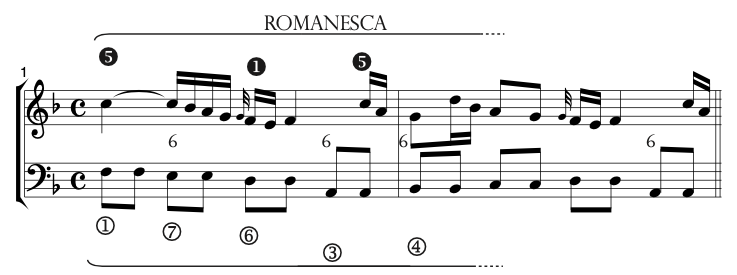
\includegraphics[scale=0.5]{hassesolfeggi.png}
\end{center}
\item Sammartini, Psalm (J-C105), mvt. 6, Gloria Patri, Andante (1750s)
\begin{center}
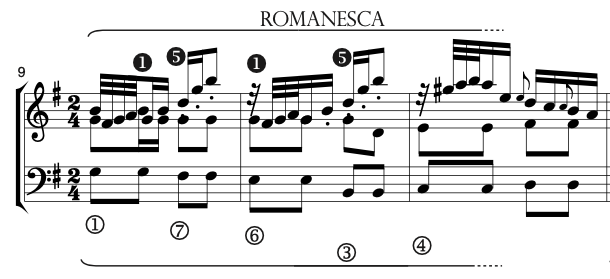
\includegraphics[scale=0.5]{sammartini105.png}
\end{center}
\end{itemize}


	\subsection{Romanesca (Old)}
	
\subsubsection{Formal description:}
\begin{itemize}
\item Number of stages: fixed in the prototype; 4 events
\item Number of voices: 2-4
\item Mode: major
\item Harmonic signature: \texttt{I V vi III}
\end{itemize}

\paragraph{Prototype:}
\begin{itemize}
\item 2 voices: \texttt{“oldromanesca.2”}
	\begin{center}
	\textbf{[[1, 3], [5, 2], [6, 1], [3, 7]]}
	\end{center}
\item 3 voices: \texttt{“oldromanesca.3”}
	\begin{center}
 	\textbf{[[1, 1, 3], [5, 7, 2], [6, 6, 1], [3, $\sharp$5, 7]]}
 	\end{center}
\end{itemize}

\paragraph{Features:}
\begin{itemize}
\item Bass:  alternating between leaping and stepwise motion
\item Parallel thirds or tenths between the upper voices
\item Ending on a major chord
\end{itemize}

\subsubsection{Examples:}
\begin{center}
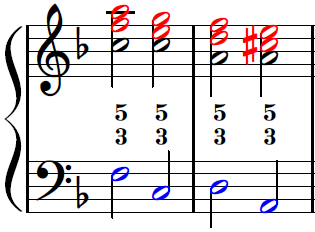
\includegraphics[scale=0.8]{oldromanesca.png}
\end{center}


	\subsection{Sol-Fa-Mi}
	
\subsubsection{Formal description:}
\begin{itemize}
\item Number of stages: 4; fixed in the prototype
\item Number of voices: 2-4
\item Mode: major / minor
\item Harmonic signature: \texttt{I ii V I}
\end{itemize}

\paragraph{Prototype:}
\begin{itemize}
\item 2 voices: \texttt{“solfami.2”} / \texttt{“solfami.2.min”}
	\begin{center}
	\textbf{[[1, 5], [2, 4], [7, 4], [1, 3]]}
	\end{center}
\item 3 voices: \texttt{“solfami.3”} / \texttt{“solfami.3.min”}
	\begin{center}
	\textbf{[[1, 3, 5], [2, 5, 4], [7, 5, 4], [1, 5, 3]]}
	\end{center}
\end{itemize}

\paragraph{Features:}
\begin{itemize}
\item Four events presented as two pairs at analogous positions in the metrical grid.
\item Melody: descending by whole step (5-4) answered by a 4-3 descent.
\item Bass : ascending 1-2 (sometimes 1-5)  answered by a 7-1 ascent (sometimes 5-1) 
\end{itemize}

\paragraph{Variants:}
\begin{itemize}
\item 1-5 bass: \texttt{“solfami.2.1-5bass”} / \texttt{“solfami.2.1-5bassmin”}
	\begin{center}
	\textbf{[[1, 5], [5, 4], [7, 4], [1, 3]]}
	\end{center}
\item cadential bass : \texttt{“solfami.2.cadbass”} / \texttt{“solfami.2.cadbassmin”}
	\begin{center}
	\textbf{[[1, 5], [2, 4], [5, 4], [1, 3]]}
	\end{center}
\item Chromatic: \texttt{“solfami.2.chromatic”} / \texttt{“solfami.2.chromaticmin”}
	\begin{center}
	\textbf{[[1, 5], [2, $\sharp$4], [7, 4], [1, 3]]}
	\end{center}
\end{itemize}

\subsubsection{Examples:}
\begin{itemize}
\item Leduc, Op.4, no.2, mvt.1, Moderato (1771)
\begin{center}
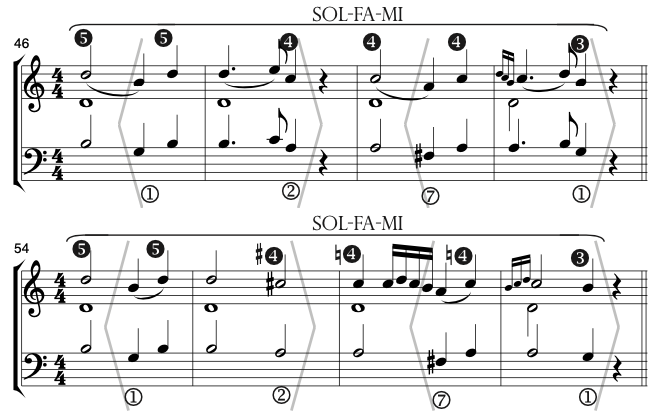
\includegraphics[scale=0.5]{leduc4.png}
\end{center}
\item Tartini, Op.6, no.4, mvt.1, Adagio (1748)
\begin{center}
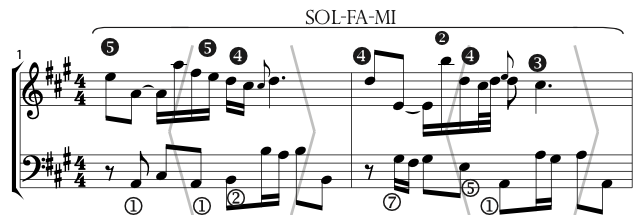
\includegraphics[scale=0.5]{tartini6.png}
\end{center}
\item Pugnani, Op.8, no.2, mvt.3, Amoroso (1774)
\begin{center}
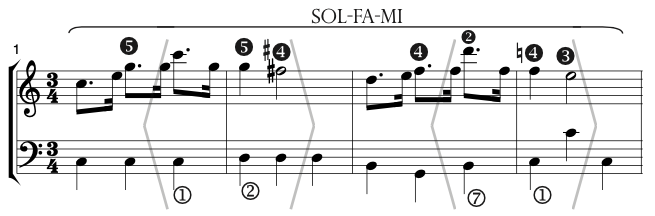
\includegraphics[scale=0.5]{pugnani8.png}
\end{center}
\end{itemize}


	\subsection{Teufelsm\"uhle}
	
\subsubsection{Formal description:}
\begin{itemize}
\item Number of stages: 6; not fixed in the prototype
\item Number of voices: 2-4
\item Mode: minor
\item Harmonic signature: \texttt{viio7/V i64 It6} (repeated one minor third higher or lower; sequential continuation)
\end{itemize}

\paragraph{Prototype (ascending):}
\begin{itemize}
\item 2 voices: \texttt{“teufelsmuehle.2.asc”}
	\begin{center}
	\textbf{[[$\sharp$4, 3], [5, 3], [$\flat$6, 3]]}
	\end{center}
\item 3 voices: \texttt{“teufelsmuehle.3.asc”}
	\begin{center}
	\textbf{[[$\sharp$4, 1, 3], [5, 1, 3], [$\flat$6, 1, 3]]}
	\end{center}
\end{itemize}

\paragraph{Prototype (descending):}
\begin{itemize}
\item 2 voices: \texttt{“teufelsmuehle.2.desc”}
	\begin{center}
	\textbf{[[$\flat$6, 3], [5, 3], [[$\sharp$4, 3]]}
	\end{center}
\item 3 voices: \texttt{“teufelsmuehle.3.desc”}
	\begin{center}
	\textbf{[[$\flat$6, 1, 3], [5, 1, 3], [$\sharp$4, 1, 3]]}
	\end{center}
\end{itemize}

\paragraph{Features:}
\begin{itemize}
\item Real-life examples can begin anywhere in the pattern
\end{itemize}

\subsubsection{Examples:}


	\subsection{Volta}
	
\subsubsection{Formal description:}
\begin{itemize}
\item Number of stages: 4; fixed in the prototype
\item Number of voices: 2-3
\item Harmonic signature: \texttt{viio64/V V6 viio I}
\end{itemize}

\paragraph{Prototype:}
\begin{itemize}
\item 2 voices: \texttt{"volta.2"}
	\begin{center}
	\textbf{[[1, $\sharp$4], [7, 5], [7, 4], [1, 3]]}
	\end{center}
\item 3 voices: \texttt{"volta.3"}
	\begin{center}
	\textbf{[[1, 2, $\sharp$4], [7, 2, 5], [7, 2, 4], [1, 1, 3]]}
	\end{center}
\end{itemize}

\paragraph{Features:}
\begin{itemize}
\item Pairwise of organization of events
\item Relation to the Quiescenza: reversal of the two pairs of chords
\end{itemize}

\subsubsection{Examples:}
\begin{center}
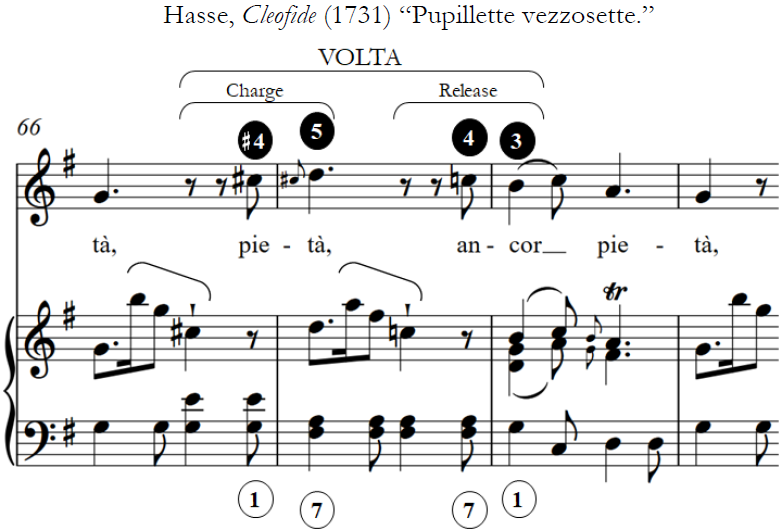
\includegraphics[scale=0.5]{volta.png}
\end{center}


	\subsection{Waldstein}
	
\subsubsection{Formal description:}
\begin{itemize}
\item Number of stages: 4; fixed in the prototype
\item Number of voices: 2-3
\item Mode: major
\item Harmonic signature: \texttt{I V6 bVII IV6}
\end{itemize}

\paragraph{Prototype:}
\begin{itemize}
\item 2 voices: \texttt{“waldstein.2”}
	\begin{center}
	\textbf{[[1, 5], [7, 5], [$\flat$7, 4], [6, 4]]}
	\end{center}
\item 3 voices: \texttt{“waldstein.3”}
	\begin{center}
	\textbf{[[1, 3, 5], [7, 2, 5], [$\flat$7, 2, 4], [6, 1, 4]]}
	\end{center}
\end{itemize}

\paragraph{Features:}
\begin{itemize}
\item Bass: chromatically descending from 1 to 6
\item Middle voices: shadows bass in parallel thirds or tenths
\end{itemize}

\subsubsection{Examples:}
\begin{center}
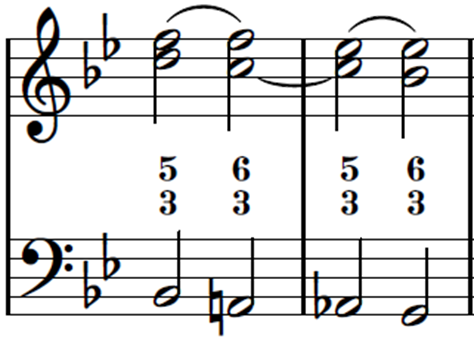
\includegraphics[scale=0.4]{waldstein.png}
\end{center}





\end{document}
